\let\negmedspace\undefined
\let\negthickspace\undefined
\documentclass[journal]{IEEEtran}
\usepackage[a5paper, margin=10mm, onecolumn]{geometry}
\usepackage{lmodern} 
\usepackage{tfrupee} 
\setlength{\headheight}{1cm}
\setlength{\headsep}{0mm}   

\usepackage{gvv-book}
\usepackage{gvv}
\usepackage{cite}
\usepackage{amsmath,amssymb,amsfonts,amsthm}
\usepackage{algorithmic}
\usepackage{graphicx}
\usepackage{textcomp}
\usepackage{xcolor}
\usepackage{txfonts}
\usepackage{listings}
\usepackage{enumitem}
\usepackage{mathtools}
\usepackage{gensymb}
\usepackage{comment}
\usepackage[breaklinks=true]{hyperref}
\usepackage{tkz-euclide} 
\usepackage{listings}                             
\def\inputGnumericTable{}                                 
\usepackage[latin1]{inputenc}                                
\usepackage{color}                                            
\usepackage{array}                                            
\usepackage{longtable}                                       
\usepackage{calc}                                             
\usepackage{multirow}                                         
\usepackage{hhline}                                           
\usepackage{ifthen}                                           
\usepackage{lscape}
\usepackage{xparse}

\bibliographystyle{IEEEtran}

\title{2.5.25}
\author{EE25BTECH11059 - Vaishnavi Ramkrishna Anantheertha}

\begin{document}
\maketitle

\renewcommand{\thefigure}{\theenumi}
\renewcommand{\thetable}{\theenumi}

\numberwithin{equation}{enumi}
\numberwithin{figure}{enumi} 

\textbf{Question}:
If $\mathbf{a} = 2\hat{i} - \hat{j} - 2\hat{k}$ and $\mathbf{b} = 7\hat{i} + 2\hat{j} - 3\hat{k}$, then express $\mathbf{b}$ in the form $\mathbf{b} = \mathbf{b}_1 + \mathbf{b}_2$, where $\mathbf{b}_1$ is parallel to $\mathbf{a}$ and $\mathbf{b}_2$ is perpendicular to $\mathbf{a}$.
\\
\textbf{Solution: }\\
\begin{table}[H]    
  \centering
  \begin{tabular}{|c|c|}
\hline
\textbf{Variable} & \textbf{Value} \\
\hline
$A$ & $(0,-\frac{3}{2})$ \\
\hline
$m$ & $\frac{1}{2}$ \\
\hline
\end{tabular}
  \caption{Variables Used}
  \label{tab:1.10.25}
\end{table}

\begin{align}
                                     \vec{a}= \myvec{
                                             2
                                              \\
                                              -1
                                               \\
                                               -2
                                              }
\end{align}
\begin{align}
                                     \vec{b}= \myvec{
                                             7
                                              \\
                                              2
                                               \\
                                               -3
                                              }
\end{align}
Using the Gram-Schmidt approach\\
$\vec{{b}_1}$ is the projection of $\vec{b}$ on $\vec{a}$
\begin{align}
  \vec{{b}_1} = \frac{\vec{a^T} \vec{b}}{\vec{a^T} \vec{a}}  \vec{a}
\end{align}
\begin{align}
\vec{{b}_1}=\frac{18}{9} \vec{a}\\
\vec{{b}_1}=2\vec{a}\\
\vec{{b}_1}= \myvec{
                     4
                     \\
                     -2
                      \\
                      -4
                           }\\
\vec{b}=\vec{{b}_1}+\vec{{b}_2}\\
\vec{b}_2 = \vec{b} - \vec{b}_1 
= \myvec{
7 \\ 2 \\ -3
}
-
\myvec{
4 \\ -2 \\ -4
}
= \myvec{
3 \\ 4 \\ 1}\\
 \myvec{
7 \\ 2 \\ -3
}
=
\myvec{
4 \\ -2 \\ -4
}
+
 \myvec{
3 \\ 4 \\ 1}
\end{align}
Therefore,
\begin{align}
  \vec{{b}_1}=\myvec{
4 \\ -2 \\ -4
}\\
\vec{{b}_2}= \myvec{
             3 \\ 4 \\ 1  }
\end{align}


Refer to Figure

\begin{figure}[H]
\begin{center}
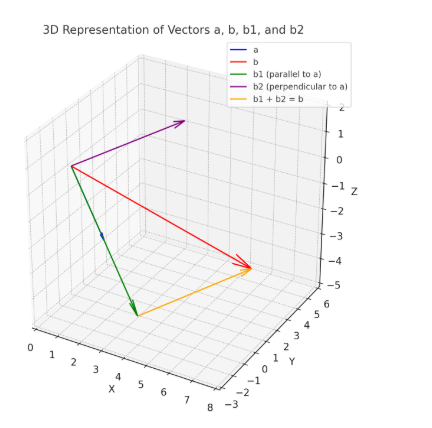
\includegraphics[width=0.6\columnwidth]{figs/Graph3.png}
\end{center}
\caption{}
\label{fig:Fig}
\end{figure}
\end{document}  